% tex file for discussion
\par \indent Cohen's paper identifies sixteen regions of brain activation 
during the course of the BART study. In particular, we were also able to detect 
high activity in the dorsal lateral prefrontal cortex, which is near the front 
of the brain. The prefrontal cortex encompasses the frontal lobe and stores 
the brain's short-term memory. Another active region of the brain highlighted 
by Cohen that we were somewhat able to identify was the bilateral occipital 
pole and cortex, near the rear of the brain. The occipital lobe is responsible 
for processing visual information. We were not able to consistently detect
the occipital lobe in our analysis. However, both active regions are showcased 
for Subject 23 in Figure \ref{fig:clustersub23}.

\begin{figure}[ht]
\centering
	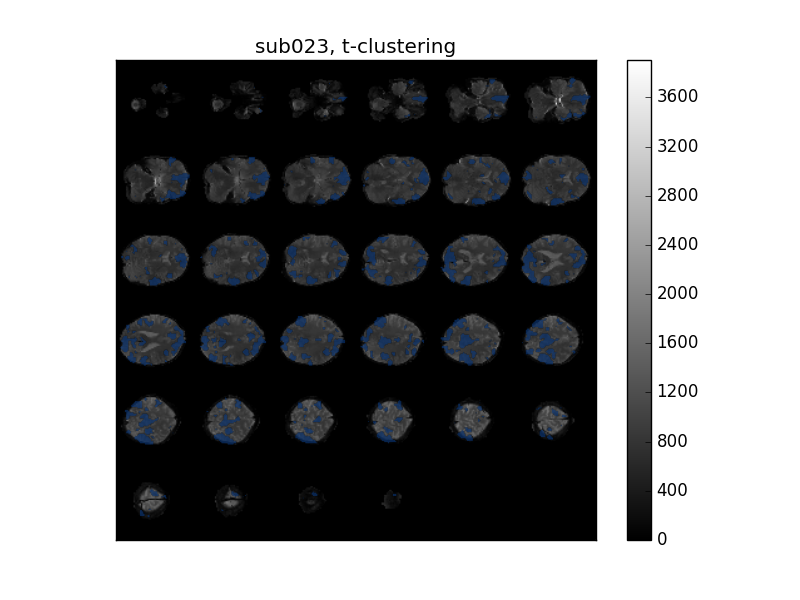
\includegraphics[width=.8\linewidth]{../images/sub023_t_overlay.png} 
	\caption{Quantile-based clustering for Subject 23's t-statistics.}
	\label{fig:clustersub23}
\end{figure}

\par BART studies measure risk-taking behavior, which is a sub-area of 
self-control. The high activity found in the prefrontal cortex is 
unsurprising, since we expect study participants to rely heavily on their 
short-term memory capabilities when trying to decide whether to keep pumping 
the balloon or the cash out. When making this choice at every step of the 
study, the subject must recall information stored in short-term memory, such 
as recollection of how many pumps it took before the balloon to explode in 
previous trials. However, the activity in the occipital lobe is less 
rationalizable in the context of risk-taking and self-control. Instead, it may 
be a side-effect of the visual aspect of the BART study, which involves 
subjects watching a computerized balloon grown in size and popping. While 
visual stimulus is not something that the BART study is interested in 
assessing, it is reasonable that the occipital lobe was nevertheless an site 
of high activity, since there was a strong visual aspect to the study. 

